\documentclass[12pt]{article}

% PACKAGES
\usepackage[utf8]{inputenc}
\usepackage{amsmath}
\usepackage{amssymb}
\usepackage{float}
\usepackage{graphicx}
\usepackage{enumerate}
\usepackage{mathtools}
\usepackage{hyperref}

% CUSTOM STYLES
\providecommand{\e}[1]{\ensuremath{\times 10^{#1}}}
\DeclarePairedDelimiter\abs{\lvert}{\rvert}%
\restylefloat{table}

% METADATA
\title{FPGA implementation of Cooley-Tukey}
\date{September 13, 2014}
\author{Garrett Massman and Cory Walker}

\begin{document}

  \maketitle

  \subsection*{Overview}
    In this project we will implement the Cooley-Tukey FFT algorithm on a Xilinx FPGA using VHDL.
  \subsection*{Theory}
    Describe the definitions of the DFT and the Cooley-Tukey FFT.
  \subsection*{In Mathematica}
    Describe Mathematica code, how precomputed tables can help us.
  \subsection*{FPGA considerations}
    Describe how we plan to utilize SPI for communication, what type of logical blocks we will use and how they will work together.
  \subsection*{Block diagram}
    Over the past few weeks we have taken what we know and outlined a basic block diagram of our device:
    \begin{figure}[H]
      \centering
      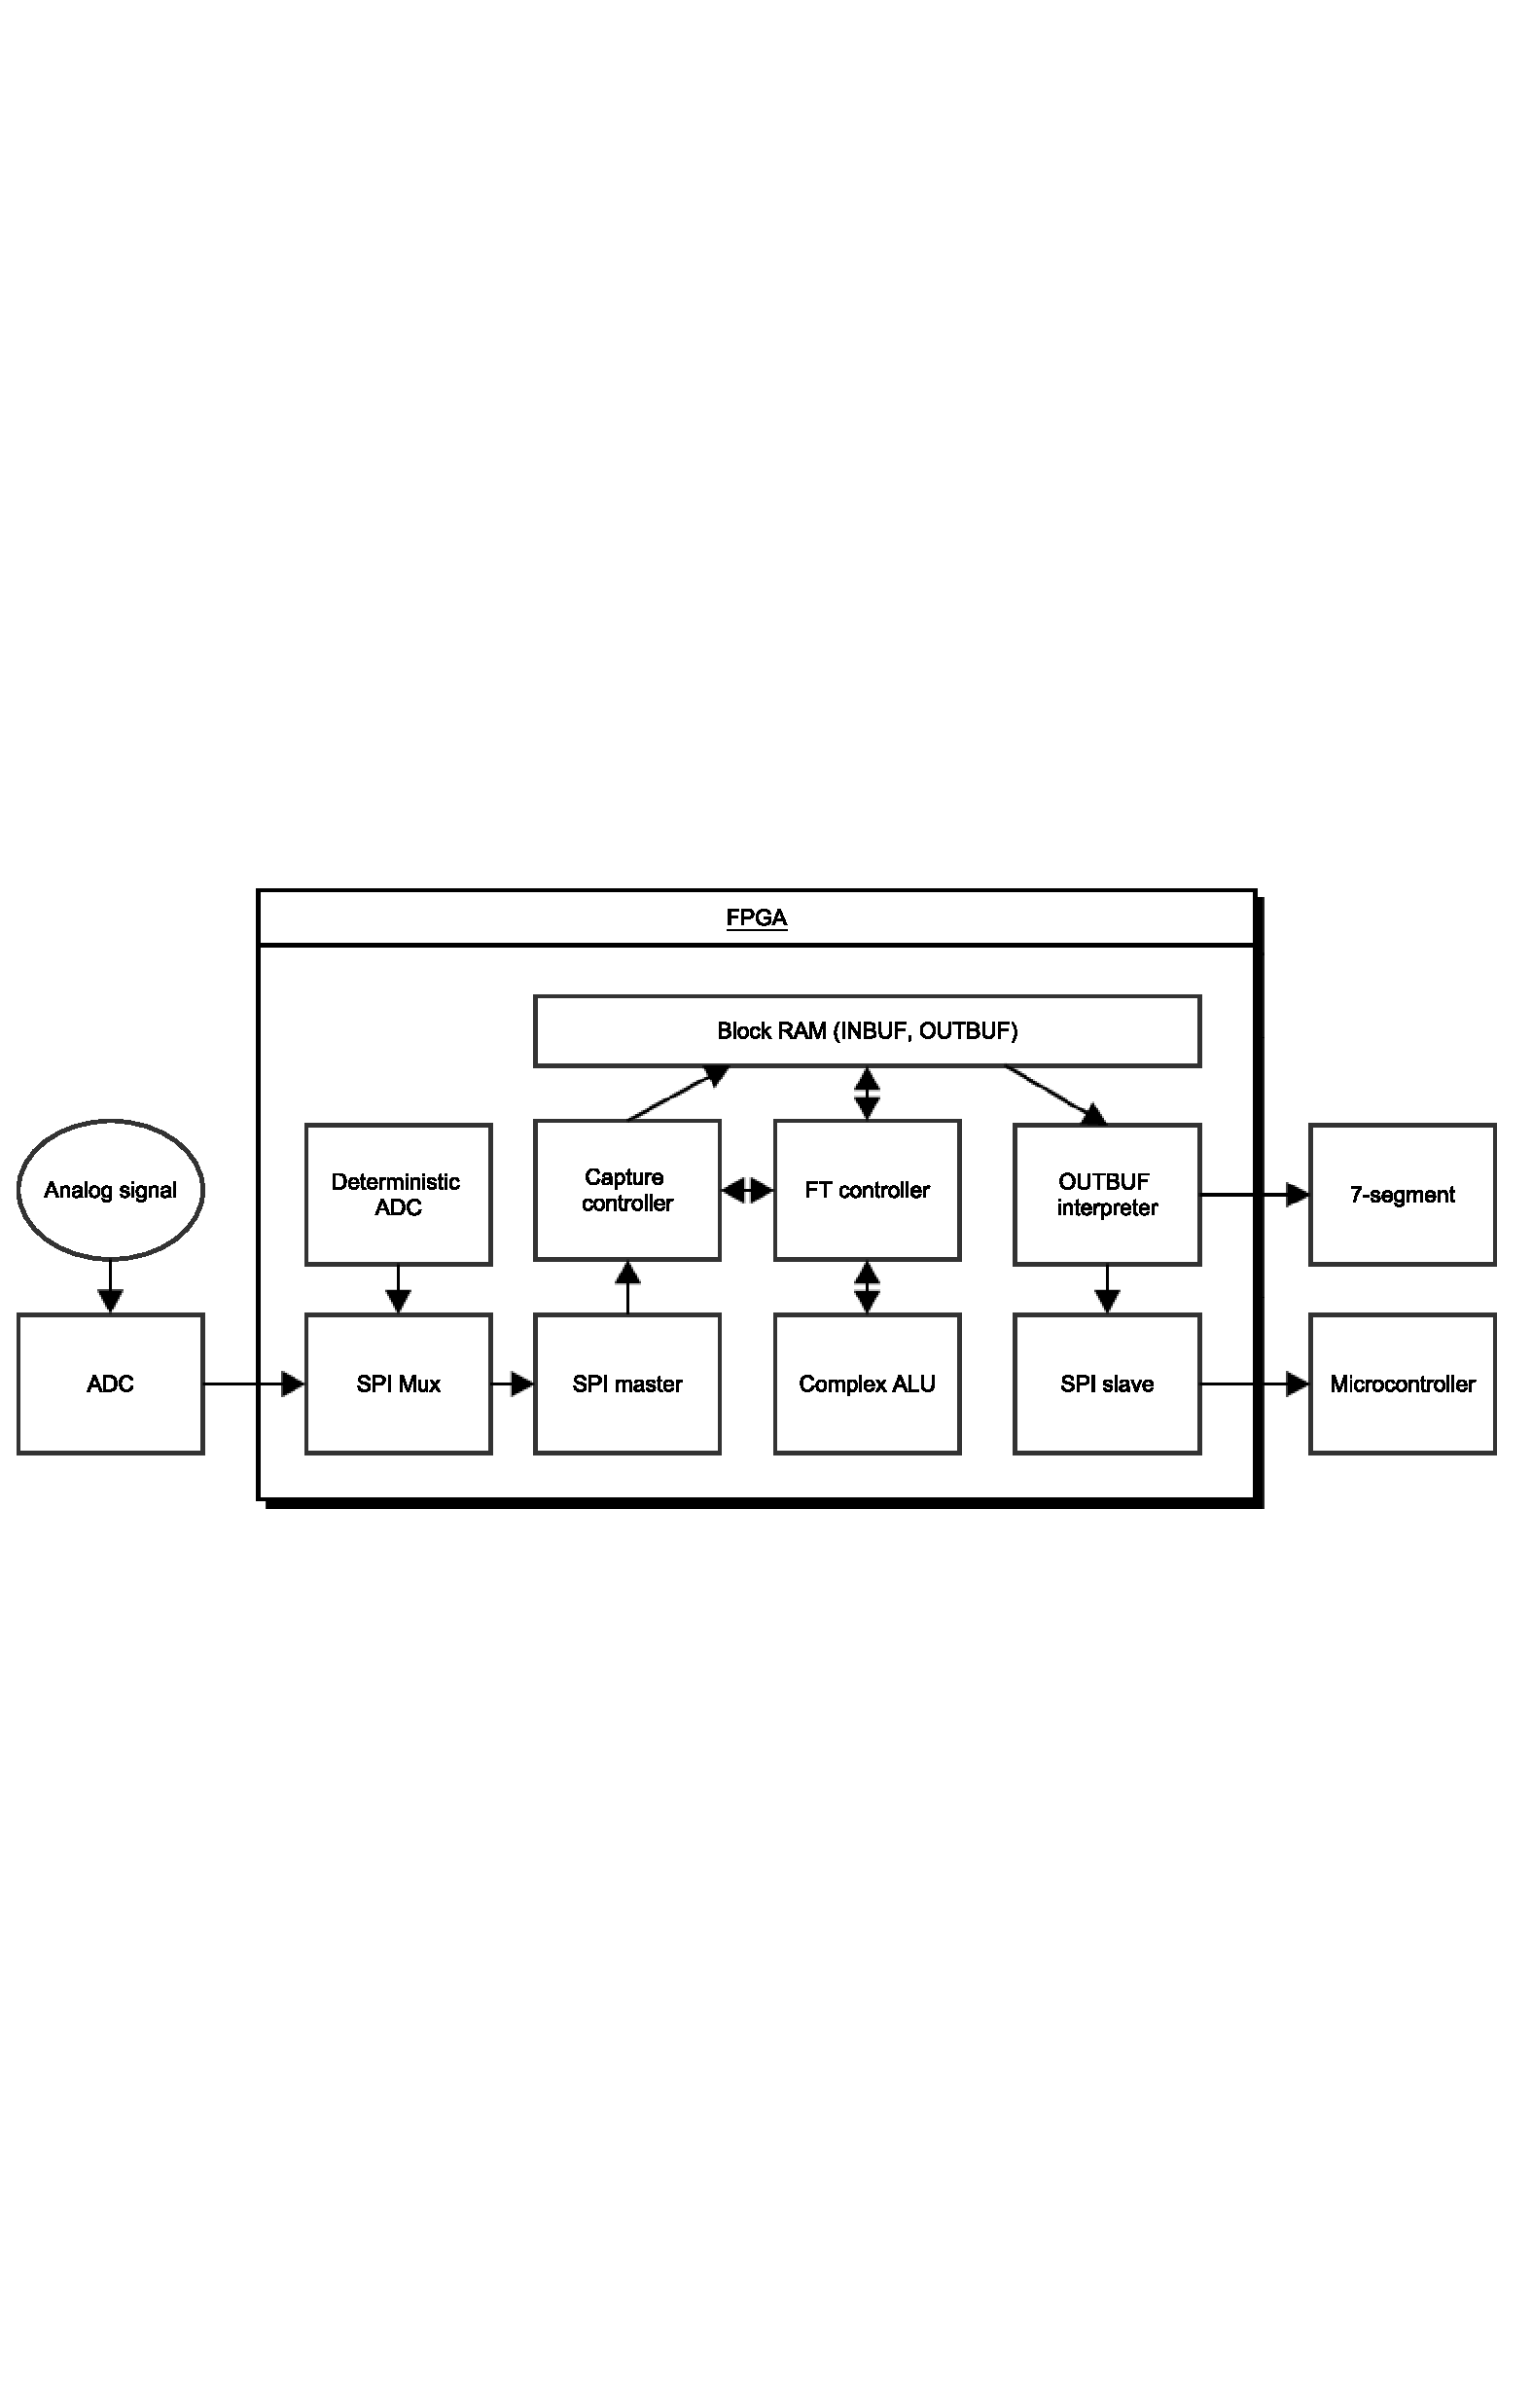
\includegraphics[trim=0 400 0 400,clip,width=140mm]{vhdl_fft.pdf}
      \caption{Block diagram of the FFT chip}
      \label{overflow}
    \end{figure}
    Now that we have divided the device into several logical blocks, we can now split up the work accordingly.
  \subsection*{Roadmap}
    Describe the steps, in order, that need to be done.
  \subsection*{Resources}
    List of resources that we plan to use.
    %http://opencores.org/project,spi_master_slave
  \subsection*{Possible extensions}
    Describe the extra things we might add if we have time.
  \subsection*{Conclusion}

  \begin{thebibliography}{9}
    \bibitem{doin}
      Doin, Jonny. \emph{SPI Master/Slave Interface.} OpenCores, 16 May 2011. Web. 13 Sept. 2014. \textless\url{http://opencores.org/project,spi_master_slave}\textgreater.
    \bibitem{reynwar}
      Reynwar, Ben. \emph{FFT on an FPGA.} FFT on an FPGA. N.p., n.d. Web. 13 Sept. 2014. \textless\url{http://www.reynwar.net/ben/docs/fft_dit/index.html}\textgreater.
    \bibitem{satoh}
      Satoh, Keiichi, Jubee Tada, Kenta Yamaguchi, and Yasutaka Tamura. \emph{Complex Multiplier Suited for FPGA Structure.} Computers and Communications (2008): 341-44. Web. 13 Sept. 2014.
    \bibitem{tukey}
      Wikipedia contributors. \emph{Cooley–Tukey FFT algorithm.} Wikipedia, The Free Encyclopedia. Wikipedia, The Free Encyclopedia, 27 Jun. 2014. Web. 13 Sep. 2014.
    \bibitem{dft}
      Wikipedia contributors. \emph{Discrete Fourier transform.} Wikipedia, The Free Encyclopedia. Wikipedia, The Free Encyclopedia, 2 Sep. 2014. Web. 13 Sep. 2014.
  \end{thebibliography}

\end{document}
